\section{فصل اول}

\subsection{اصطلاحات}

\subsubsection{\lr{World problem} یا \lr{Environment}}

دنیای مسئله جایی است که مشکلی در آن رخ داده است و کسی وجود دارد که این مشکل را
در ابتدا بررسی و بعد از آن حل می‌کند. در حقیقت دنیا، محیط عملیاتی ما در مهندسی
نیازمندی است. این دنیا می‌تواند سینما باشد یا دانشگاه. جنس این مسائل می‌تواند
مشکل باشد که بایستی برطرف شود یا قابلیتی که می‌خواهیم در آینده اتفاق بیوفتد.

\subsubsection{\lr{Machine}}

ماشین راه‌حلی برای حل مسئله‌ای می‌باشد که پیش آمده است. ماشین می‌تواند به صورت
آماده خریداری شود یا توسط تیم توسعه از صفر توسعه داده شود. ما باید در سند
نیازمندی این نوع از نیازمندی را مشخص کنیم. ماشین در حقیقت نرم‌افزاری است که قرار
است داشته باشیم \footnote{\lr{Software to be}}. مدیر نیازمندی با توجه به هزینه
می‌تواند برای مهندس نیازمندی تعیین کند که آیا داشتن نرم‌افزار آماده هزینه کمتری
برایش دارد یا توسعه آن نرم‌افزار از صفر توسط تیم توسعه خود.

\subsubsection{\lr{Context}}

کلمه \lr{Context} به معنای زمینه می‌باشد. تمام رفتار‌ها و شکل‌های انجام کار را
نشان می‌دهد. مشخص می‌کند که چه نیازمندی‌های علمی را باید بدانیم تا بتوانیم در
نرم‌افزار آن را پیاده‌سازی کنیم. زمینه‌های مرتبطی برای توسعه‌ که باید به علوم
آنها واقف شویم. برای مثال هنگام توسعه یک نرم‌افزار تشخیص پیوند مولکولی و طراحی
پروتئین نیازمند آن هستیم که در مورد شاخه‌های علمی بایولوژی، بایوتک و ژنتیک علومی
را کسب کنیم. این علوم می‌تواند توسط تحقیقات و پژوهش‌های فردی بدست آید یا اینکه
در راستای تحصیل در یک رشته می‌توانیم در رشته دیگر به تحصیلات آکادمیک بپردازیم و
به نوعی مدرک کارشناسی آن حوزه را بدست آوریم که بتوانیم به صورت کامل روی موضوع
عملیاتی خود واقف و مسلط شویم.

\subsubsection{\lr{Statement} یا جمله}

\lr{Statement} یک جملست که ترکیبی از پدیده‌ها می‌باشد. برای مثال گفته می‌شود،
وقتی ترمز خودرو فشرده شد، در‌ها قفل شود و کاربر بتواند وضعیت دنده خود را تغییر
دهد. بعضی از این پدیده‌ها در دنیای مسئله یا محیط اتفاق می‌افتد. فعل‌های محیطی را
به هم متصل می‌کند و به فعل‌های نرم‌افزاری دخالتی ندارد.

\subsubsection{\lr{Phenomena} یا پدیده‌ها}

تمام اتفاقاتی که در مسئله (یا جمله) رخ می‌دهد را پدیده یا \lr{Phenomena} گویند.
برخی پدیده‌ها دقیقاً داخل نرم‌افزار رخ می‌دهد، مانند خطای TLS یا خطای پیدا نشدن
صفحه. برخی پدیده‌ها بین ارتباطات رخ می‌دهد مانند نرمال‌سازی دیتابیس. پدیده خرید
کردن یک پدیده محیطی است. وقتی برای کاربر اعلانی ارسال می‌شود در واقع این اعلانات
پدیده‌ بین محیط و نرم‌افزار است.

\subsubsection{\lr{System as is}}

سیستمی که در حال حاضر وجود دارد سیستم جاری یا \lr{System as is} گویند. سیستم
جاری بیشتر به محیط مربوط است. به عبارتی دیگر، المان‌ها و ارتباطاتی است که الان
وجود دارد مانند افراد و دستگاه‌ها.

\subsubsection{\lr{System to be}}

\lr{System to be} دقیقاً سیستمی است که در آینده خواهیم داشت. تمام فرایند مهندسی
که منجر به تولید سیستمی جدید می‌شود. چیزی که باید رخ دهد. مجموعه‌ای از المان‌های
محیطی و \lr{Software to be}.

\subsubsection{عوامل \lr{Prescriptive}}

عواملی که تجویزی هستند که نیاز سیستم را مشخص می‌کنند که چه کاری باید انجام شود:

\begin{enumerate}
    \item \lr{System requirement}: یک \lr{System requirement} مجموعه‌ای از
    \lr{Assumption}ها و \lr{Software requirement}هاست. تمام تک کار‌های کوچکی که
    به محیط اختصاص می‌دهیم.
    \item \lr{Software requirement}: تمام نیازمندی‌های نرم‌افزاری که می‌تواند به
    دو دسته \lr{Functional} و \lr{Non-functional} تقسیم شود. تمام تسک‌های کوچکی
    که به نرم‌افزار اختصاص می‌دهیم.
    \item \lr{Assumption}: تمام عوامل محیطی که در پایین توضیح داده شده است.
\end{enumerate}

مثال‌هایی از انواع \lr{System requirement}:

\begin{itemize}
    \item تمام در‌های قطار بایستی در هنگام حرکت بسته باشند.
    \item مشتریان هیچ وقت نمی‌توانند بیشتر از سه کتاب را در یک زمان قرض بگیرند.
    \item تمام محدودیت‌های دعوت یک شرکت کننده به یک میتنینگ آنلاین بایستی به
    زودی برطرف شود.
\end{itemize}

\subsubsection{مفروضات یا \lr{Assumption}}

تمام عواملی که محیطی هستند و مستقیماً با نرم‌افزار ارتباطی ندارند. در واقعیت امر
همان محیط و یا \lr{World problem} هستند. ابزار‌هایی واسط بین انسان و انجام کار.

\begin{enumerate}
    \item \lr{People}: مردم و کاربران
    \item \lr{Device}: دستگاه‌ها مانند سنسور‌ها، جمع‌آور داده و ارسال کننده به
    موتور تحلیل (نرم‌افزار)
    \item \lr{Exists softwares} نرم‌افزار‌های موجود: نرم‌افزار‌هایی که خودشان
    عملیات متعددی انجام می‌دهند و داده‌ها را برای تحلیل به نرم‌افزار اصلی سیستم
    ما ارسال می‌کنند.
\end{enumerate}

عوامل محیطی گسترده هستند. برای مثال وقتی که کاربر در اپلیکیشن سبد خرید خود را
می‌خواهد حساب کند، زدن روی دکمه "پرداخت آنلاین" کاملا یک عامل محیطی است یعنی
\lr{Assumption}. زیرا با دخالت کاربر می‌توان سبد خرید را پرداخت کرد، در غیر این
صورت نرم‌افزار خودش نمی‌تواند تصمیم بگیرد که پرداخت نهایی را کی باید انجام دهد
(دیدگاه یک سیستم ساده).

\subsubsection{مثال}

سناریو: در‌های قطار موقع حرکت قفل شود. در این سناریو \lr{Statement}، پدیده‌ها
(Phenomena) و نیازمندی سیستم و پدیده‌های محیطی را مشخص کنید.

\begin{itemize}
    \item جمله: در‌های قطار موقع حرکت قفل شود.
    \item پدیده‌ها در این جمله دو نمونه هستند. حرکت کردن قطار و بسته شدن در‌ها
    \item عوامل محیطی یا \lr{Assumption}ها سنسور تشخیص حرکت قطار و محرک بازوی
    در‌های قطار هستند که دائماً در حال مانیتور و کنترل در‌ و حرکت قطار هستند.
    \item \lr{Assumption}ها یعنی سنسور‌های قطار و نرم‌افزاری که قوه تحلیل دارد
    یا \lr{Software requirement} می‌شود نرم‌افزاری که قرار است در آینده داشته
    باشیم یا \lr{Software to be}.
    \item کل این مجموعه را \lr{System to be} گویند.
\end{itemize}

\begin{figure}[H]
    \centering
    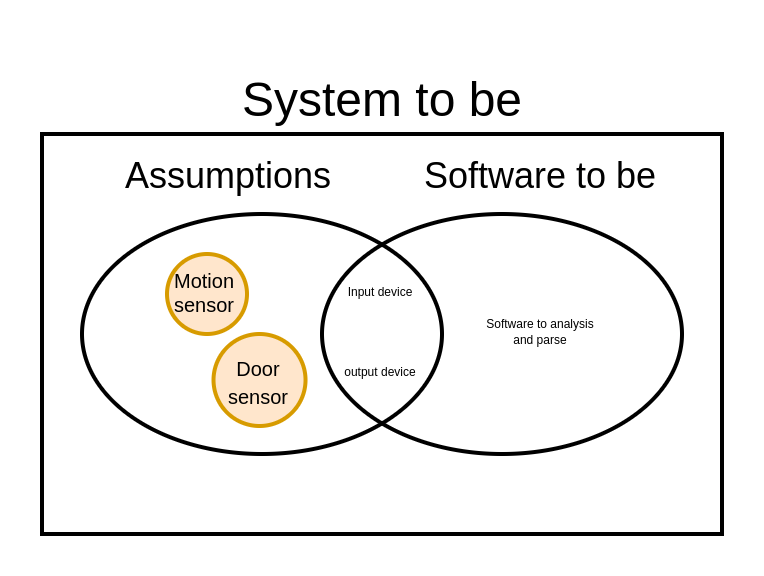
\includegraphics[width=0.5\textwidth]{images/system_to_be.png}
    \caption{مهندسی نیازمندی بیشتر به \lr{Assumption} و قسمت اشتراکی شامل می‌شود.}
    \label{fig: systemToBe}
\end{figure}

\subsubsection{مفهوم \lr{Definition}}

یک معنای دقیق از چیزایی است که می‌نویسم به عبارت دیگر تمام اصطلاحاتی که در سیستم
می‌تواند وجود داشته باشد را بیان می‌کند.

\subsubsection{مفهوم مانیتور کردن}

مانیتور کردن یعنی بررسی داده‌های ورود و انجام تحلیل روی آنها.

\subsubsection{مفهوم کنترل کردن}

کنترل کردن یعنی فرایند بعد از تحلیل، یعنی اعمال کردن نتایج بدست آمده.

\subsubsection{عوامل \lr{Descriptive}}

عوامل توصیفی، قوانین طبیعی و قید و شرط‌های فیزیک که غیر 

\subsubsection{ویژگی دامنه یا \lr{Domain property}}

یک عبارت توصیفی است که یک حقیقت از فیزیک را بیان می‌کند. این عبارت قابل مذاکره
نیست که برای مثال بگوییم بعداً می‌توان آن را تغییر داد. به هیچ وجه نمی‌توان آن
را کم یا زیاد کرد.

برای مثال:

\begin{enumerate}
    \item برای مثال دانشجو نمی‌تواند دو درس مختلف در زمان یکسان اخذ کند. یعنی از
    نظر فیزیک نمی‌توان همزمان در دو کلاس در زمان یکسان حاضر شد. و این پیام را
    نیازمندی نرم‌افزار در حقیقت برنامه نویس مشخص می‌کند.
    \item هنگامی که در‌های قطار بسته باشند، یعنی دیگر باز نیستند.
    \item اگر شتاب قطار مثبت باشد، بدان معانست که سرعت قطار =! صفر می‌باشد.
\end{enumerate}

\subsubsection{دامنه‌ها}

دامنه‌های در دل سازمان‌ها هستند، مانند دامنه پژوهشی، دامنه‌های مالی و ارتباط بین
آدم‌ها در دامنه وجود دارد.

\subsubsection{اسکوپ‌ها}

مجموعه‌هایی از \lr{System requirement} هستند که نرم‌افزار می‌تواند در آنها ورود
داشته باشد. مثلا فعالیت‌های مربوط به ثبت‌نام دانشجو، که اصطلاحاً به آنها
\lr{System scope} می‌گویند.

\subsubsection*{نکات}

\begin{itemize}
    \item مهندس نیازمندی باید در کنترل و مدیریت اسکوپ‌ها حساسیت داشته باشد که
    نرم‌افزار از دست خارج نشود و باعث پیچیده‌تر شدنش نگردد.
    \item دامنه‌ها درست است که ثابت و غیرقابل مذاکره هستند، اما از یک دامنه به
    دامنه دیگر می‌تواند ویژگی‌ها تغییر کنند در حالی که ساختار این دامنه حفظ شود.
    برای مثال زمانی که دامنه مورد نظر یک کتابخانه فیزیکی است، همزمان دو نفر
    نمی‌توانند یک کتاب مشترک را تقاضا کنند. اما در کتابخانه دیجیتال که به صورت
    اپلیکیشن می‌باشد، درست است که ساختار دامنه همانند موجودیت‌ها و شکل کتابخانه
    فیزیکی است اما نحوه استفاده آن کاملاً تغییر کرده و چندین کاربر می‌توانند
    همزمان یک کتاب را به صورت دیجیتال مطالعه کنند.
    \item در مهندسی نیازمندی تنها یک نمودار استفاده نمی‌شود. برای مثال زمانی که
    یک نمودار \lr{Sequence} برای نمایش ارتباطات دستگاه ها کشیده می‌شود نیازمند
    آن است که نمودار هدف نیز داشته باشد. بعد از آن بایستی تمام ریسک‌های مربوط به
    آن نیز به صورت نمودار اعلام شود. چرا که باعث تولید یک سند مهندسی نیازمندی
    کامل می‌شود که در زمان‌های مختلف می‌توان به آن مراجعه کرد و متوجه تمام
    موضوعات بدون فراموشی تنها یک بخش شد.
    \item بُعد \lr{Why} در نمودار معمولاً نشان‌دهنده اهداف است. مثلا پیاده‌سازی این
    قابلیت هدف‌اش رضایت مشتری است.
    \item همیشه از اهداف شروع می‌کنیم و به نیازمندی‌های سیستمی می‌رسیم و
    نیازمندی سیستمی را در نیازمندی‌های نرم‌افزاری و محیطی بررسی می‌کنیم.
\end{itemize}

\begin{figure}[H]
    \centering
    \begin{forest}
        [Goal
            [
                [System requirement
                    [
                        Software requirement
                    ]
                    [
                        Assumption
                    ] 
                ] 
                [System requirement
                    [
                        Software requirement
                    ]
                    [
                        Assumption
                    ] 
                ] 
            ]
        ]
    \end{forest}
\end{figure}

\subsubsection{تفاوت‌های بین \lr{Descriptive} و \lr{Prescriptive}}

\begin{itemize}
    \item جملات تجویزی را می‌توان برای آنها مذاکره کرد، آنها را کم و زیاد کرد یا
    حتی برای آنها جایگزینی معرفی نمود.
    \item جملات توصیفی اصلاً قابل تغییر نیستند.
\end{itemize}

\subsection{مولفه‌های مربوط به نیازمندی نرم‌افزار در نیازمندی سیستم}

\begin{enumerate}
    \item مانیتورینگ: تمام مقادیر محیطی که نرم‌افزار توسط دستگاه‌های ورودی مانند
    سنسور‌ها، داده‌های آن را دریافت می‌کند.
    \item کنترل: مقادیر محیطی که نرم‌افزار آنهارا می‌تواند از طریق دستگاه‌های
    خروجی (Actuators) آن‌ها را کنترل (اعمال) کند.
    \item مقادیر دستگاه‌های ورودی \footnote{Input}: تمام داده‌هایی که به عنوان
    ورودی در نرم‌افزار استفاده می‌شود.
    \item متغیر‌های خروجی \footnote{Output}: مقادیری که نرم‌افزار آنها را در
    دستگاه‌ّای خروجی اعمال می‌کند.
\end{enumerate}

\subsubsection*{نکته}

بیشتر سازمان‌ها به دو دسته زیر فعالیت‌های خودشان را انجام می‌دهند:

\begin{enumerate}
    \item سازمان‌هایی که هدفگرا هستند و تنها برای رسیدن به محصول آخرین تلاش و
    فعالیت خود را می‌کنند.
    \item سازمان‌هایی که تعداد \lr{Agent} و کاربرانشان زیاد است و ارزش‌های زیادی
    برای آنها قائل می‌شوند به صورت Agentگرا یا عاملگرا هستند.
\end{enumerate}

سطح \lr{System requirement} بالا می‌باشد، چرا که مشتری تنها درخواست می‌کند که
می‌خواهد چنین قابلیت‌هایی وجود داشته باشد، به ماهیت و نیازمندی و حتی پیچیدگی
آنها کاری ندارد.

\subsection{توافق بر لغات}

\begin{enumerate}
    \item \lr{SOFTREQ}: منظور \lr{Software requirement}
    \item \lr{ASM}: منظور مفروضات یا \lr{Assumption}
    \item \lr{DOM}: منظور دامنه یا \lr{Domain}
\end{enumerate}

\begin{equation}
    SOFTREQ + ASM + DOM \rightarrow SYSTEMREQ
\end{equation}

اگر نیازمندی نرم‌افزار، مفروضات و دامنه‌ها همگی مقید و راضی باشند نیازمندی سیستم
نیز بدست می‌آید. با استفاده از پارامتر‌های بالا می‌توان به سیستم نهایی رسید.

\newpage

\begin{figure}[H]
    \centering
    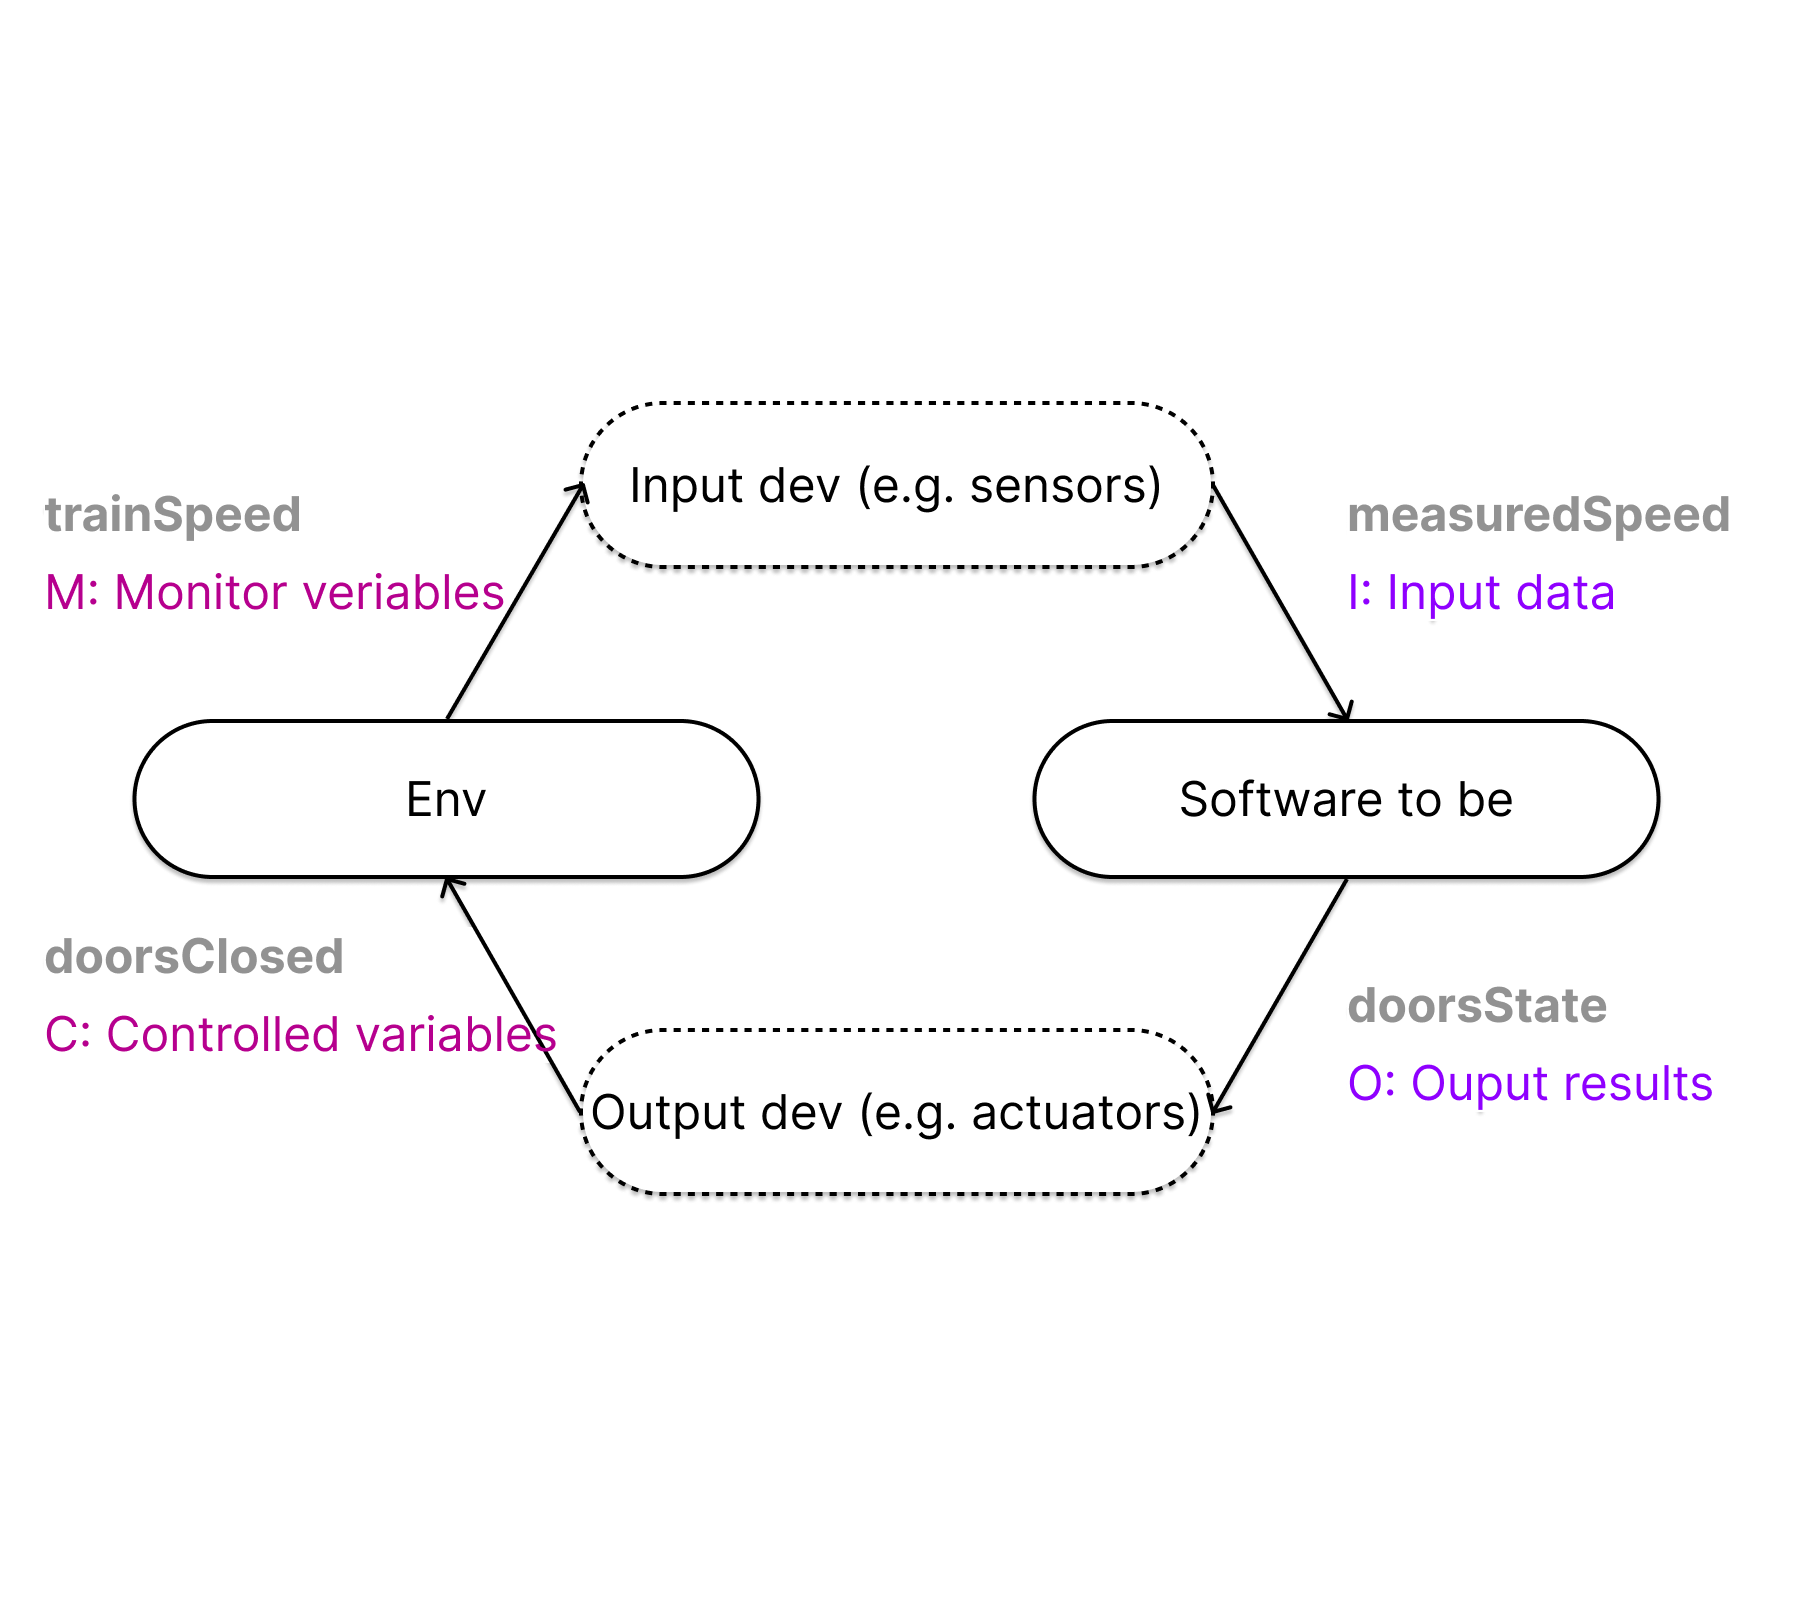
\includegraphics[width=0.7\textwidth]{images/train_sysreq.png}
    \caption{ارتباط نیازمندی سیستم در نرم‌افزار به همراه استدلال‌ها}
    \label{fig: }
\end{figure}


\begin{LTR}
    \begin{itemize}
        \item \lr{SOFTREQ}: Input ` Ouput
        \item \lr{ASM1}: Monitor ` Input
        \item \lr{ASM2}: Ouput ` Control
        \item \lr{SYSREQ}: Monitor ` Control
    \end{itemize}
\end{LTR}

\subsection*{استدلال سناریو}

\begin{equation}
    SOFTREQ: measuredSpeed \neq 0 \rightarrow doorsState = "closed"
\end{equation}

\begin{equation}
    ASM1: measuredSpeed \neq 0 iff trainSpeed \neq 0
\end{equation}

\begin{equation}
    ASM2: doorsState = "closed" iff doorsClosed
\end{equation}

\begin{equation}
    DOM: trainMoving iff trainSpeed \neq 0 
\end{equation}

\begin{equation}
    SYSREQ: trainMoving \rightarrow doorsClosed 
\end{equation}

\subsection{دسته‌بندی نیازمندی‌ها}

\subsubsection{\lr{Functional requirement}}

تعیین می‌کند که چه سرویسی قرار است در \lr{Software to be} ارائه شود. برای مثال:

\begin{itemize}
    \item نرم‌افزار کنترل قطار باید بتواند سرعت تمام بخش‌های سیستم قطار را کنترل
    کند.
    \item سیستم آنلاین فهرست کتب باید براساس موضوع کتاب نام تمام کتابخانه را
    نمایش دهد. 
    \item کاربران در سیستم پارکینگ آنلاین باید بتوانند رزرو لحظه و رزرو روزانه
    را به انتخاب خودشان استفاده کنند.
    \item دانشجویان زمانی که وارد کلاس آنلاین می‌شوند باید قابلیت به اشتراک
    گذاری صفحه نمایش خود را داشته باشند.
\end{itemize}

همچنین می‌توانند براساس شرایط محیطی باشند که تحت آن چه عملیاتی باید انجام شود:

\begin{itemize}
    \item در‌های قطار تنها در زمانی می‌توانند باز شوند که قطار به طور کامل ایستاده باشد.
\end{itemize}

\subsubsection*{دسته‌بندی توابع}

\begin{enumerate}
    \item \lr{Information}: اطلاع رسانی، اعلانات هر چیزی که قابلیت ارسال و
    دریافت را داشته باشد.
    \item \lr{Satisfaction}: تعیین \lr{State} یک کار است که در جریان معنا دارد.
    \item \lr{Stim-response}: محرک پاسخ، وقتی دکمه در \lr{UI} زده شد آلارم را
    صدا کند.
\end{enumerate}

\subsubsection{\lr{Non-functional requirement}}

تعیین می‌کنند که چگونه یک سرویس می‌تواند ارائه شود. برای این دسته باید مجموعه‌ای
از اقدامات که بار اجرایی دارند را استفاده کرد:

\begin{itemize}
    \item معیار‌ها و نیازمندی‌های کیفی:
    \begin{itemize}
        \item معیار‌های ایمنی
        \item معیار‌‌های امنیتی
        \item سرعت و دقت
        \item عملکرد زمانی و حافظه‌ای
        \item قابلیت استفاده
    \end{itemize}
    \item بقیه موارد
    \begin{itemize}
        \item هنجار‌ها
        \item معماری
        \item نیازمندی‌های توسعه 
    \end{itemize}
\end{itemize}

برای مثال:

\begin{itemize}
    \item دانشجویان هنگام به اشتراک گذاری صفحه خود کیفیت صوت را به خوبی قبل از
    اشتراک گذاری داشته باشند.
    \item قطار هنگام حرکت امکان باز کردن در را نداشته باشد.
    \item دستورات شتاب قطار هر ۳ ثانیه یکبار می‌تواند ارسال شود.
\end{itemize}

\subsection{کیفیت سرویس‌دهی یا \lr{QoS} (محصول)}

پارامتری را نشان می‌دهد که می‌خواهیم آن را از نظر کیفی تامین کنیم. برای مثال
برقراری اهداف امنیتی.

\subsection{\lr{Service Level Agreement}}

یک توافق بین معمار نرم‌افزار و کارفرما برای تعیین سطح سرویس از نظر کیفی می‌باشد.
در قرار‌داد‌های \lr{SLA} مقدار قابل قبولی از \lr{QoS}هایی که دنبالش هستیم را
بیان می‌کنیم.

\subsection{تفاوت بین \lr{Constraint} و \lr{Limitation}}

\lr{Constraint} به معنای قید و شرط است، مقید شدن به چیزی. برای مثال نرم‌افزاری
توسعه داده شود که قابلیت نصب روی دستگاه‌های موبایل را داشته باشد.

\lr{Limitation} به معنای محدودیت است که بار منفی دارد. در این حالت نرم‌افزار
باید با آن کنار بیاید.

\subsection{مفهوم هنجار‌ها یا \lr{Compliance} (محصول)}

منظور از \lr{Compliance} قواعد و هنجار‌هایی است که الزاما ثابت نیستند. نرم‌افزار
باید تابع این هنجار‌ها باشد. قواعدی که در نرم‌افزار قید می‌شود برای مثال فاصله
بین دو ماشین در سال ۲۰۲۰ با تصمیم‌گیری شهرداری برای ماشین‌های خودران ۴ متر توافق
شد. اما بعد از پیشرفت تکنولوزی و علوم مربوطه این فاصله به یک متر کاهش یافت.

\subsection{قید‌های معماری \lr{Architectural constraint} (محصول)}

بعضی از قید‌های معماری مربوط به نصب و راه‌اندازی هستند و برخی دیگر مربوط به
توزیع می‌باشند.

\begin{enumerate}
    \item نصب
    \begin{enumerate}
        \item نرم‌افزار باید روی پلتفرم موبایل یا عینک گوگل قابل نصب باشد
        \item مشخصات لازم برای نصب موفقیت‌آمیز نرم‌افزار و بازی
        \item این نیاز می‌تواند پایین‌تر از سطح سکو نیز باشد، مثلاً نصب تنها در
        یک سیستم عامل مخصوص
        \item قابلیت نصب تنها در سخت‌افزار‌های X86
    \end{enumerate}
    \item قید توزیع: ورودی و خروجی از دو درب مختلف در دانشگاه، به دلیل آنکه
    داده‌های محیطی ورودی و خروجی در دو محل متفاوت است برای رسیدن به توافق در این
    توزیع باید این داده‌ها را در یک جا با هم سینک کنیم تا اطلاعات ورودی و خروجی
    مناسب یکدگیر پدید آید.
\end{enumerate}

\subsection{قید‌های توسعه \lr{Development constraint} (مدیر پروژه)}

یکی از مهم‌ترین عوامل نگرانی مدیر پروژه است، کاری به ماهیت محصول ندارد بلکه برای
او مهم‌ترین عوامل انتخاب مناسب متدولوژی و تصمیم درست می‌باشد. تعیین هزینه زمانی
و مالی نیز از دیگر نگرانی‌های مدیر پروژه می‌باشد تا در نهایت طراح معماری بتواند
با دید کامل و بدون تحت فشار قرار گرفتن، معماری مناسب را طراحی کند.

جلسه چهارم:


کیفیت جمله‌ها میتواند صرفا کیفیت درستی نداشته .

مجموعه ای از قابلیت‌ها میشه اسکوپ که در دامین‌ها تعریف می‌شوند.

برای ساخت سبد باید فرایند‌های مهندسی نیازمندی را برویم:

چهار قدم مهندسی نیازمندی:

تمام مراحل تکرار پذیر هستند.

ساعت گرد. داده‌ها جمع‌آوری میشود ولی همه داده‌ها انتخاب نمی‌شود. یکی از آنها
انتخاب می‌شود.

دامنه و استخراج نیازمندی‌ها

ارزیابی و توافق

ممکنه چیزایی جمع‌اوری کرده باشیم که کاملا نامربوط به اسکوپ باشد. هر آنچه به ما
می‌گویند ممکنه ریسک‌هایی باشد کگه می‌ةواند قابلیت بخش به نرم‌افزار باشد.

مثلا ریسک این وجود دارد که ممکنه اینترنت قطع بشود.

نیازمندی‌هایی که به ما وارد میکند الزاما همراستا نیست

میخواهد کارنامه ببیند دانشجو، استاد میگه ثبت نمره میخوام کارنامه رو ببینم. 
اگه یکی رو برآورده کنیم ممکنه کانفلیکت به وجد آید.

اولویت نیازمندی ها را آیا تعین کرده‌ایم؟ لیست دروس رو نشون ندیم ولی دانشجو
بتواند درس انتخاب کند. (امکان ندارد.)

همه این تصمیمات رو باید ارزیابی کنیم.

دسته آخر: یک سبدی که خیلی آشفته بود تبدیل به سبدی میشود که همه روی آن توافق
دارند و به طراح داده‌میشود.

نیازمندی‌هایی که روی آنها توافق شده است.

سبد بعد از آن به طراح تحویل داده می‌شود که زبان مشترک بین طراح و نیازمندی میشه
اشکال بصری که مطالب صریح و سریع انتقال شود.

سند یک قالب می‌خواد که استاندارد است. با چی بنویسیم با نماد گرافیکال نمایش بده.

بخش آخر:

ادغام، اعتبارسنجی:
سبد دستخوش تغییرات است. تا برسد به ۸۰ درصد ثابت و ۲۰ درصد تغییر کننده. این تغییر
۲۰ درصدی می‌تواند ساید افکت ایجاد کند. پس برای رفع ساید افکت باید اعتبارسنجی
حتما انجام شود.

می‌تواند چندین دور بزد.

اسلاید ۵۲:

آیا هر سیستمی نیازمند مهندسی نیازمندی است؟ خیر. 

سیستم‌های لگیسی حتما سند نیازمندی می‌خواهند. 

کلا اونایی که ورکفلو‌های اصلی رو می‌چرخونن سند نیازمندی می‌خواد

پروژه‌های استارتآپی که قراره خدمات به مردم بده که جنس خدمت یکیه و نحوه انجام آن
متفاوت است. این سیستم‌ها هم سند نیازمندی براشون اهمیت داره.

سند نیازمندی قابلیت reuse را به پروژه‌های مشابه می‌دهد.

یک مبنعی برای پروژه‌های مشابه میشه نه یه الگو.

اسلاید ۵۲

سند نیازمندی: اول خواسته در آورده می‌شه بعد قرارداد پروژه در میاد.

سازمان‌ها براسساس Request for proposal کار میکنند. که مهندس نیازمندی و متخصصین
اوجنا می‌نویسن که معمولا واحد‌های it مسئول آنها هستند.

پروتوتایپ در خصوص بخری نیازمندی‌ها که مبهم است که واضح نیست یک پروتوتایپ درست
می‌کنیم که بفهمیم اون نیاز چیست. می‌تواند روی کاغذ باشد باشد یا یه ui اشد. که
منظور اولیه رو برساند. می‌تواند تو سطح فاکنشن باشد هم می‌تواند نان فانکشن باشد.

چرا این سند دو طرفه‌است. توی محیط یه چیزی به ما گفتن. یعنی یه نیازی به ما منقل
شده که ما پروتوتایپ درست کردیم. بعد اون پروتوتایپ رو بهش نشون میدیم که ببینیم
درست فهمیدیم یا نه. ممکن نیازمندی اضافه بشه یا حذف بشه تا سبد اسکوپ ما کامل شود.

تخمین پروژه: باید سند نیازمندی‌ها دیده شود که بفهیمیم چقدر خواسته داریم تا زمان
مشخص کنیم، تا هزینه و اندازه تخمین بزنیم. ورژن بندی اینجا انجام می‌شود. یکی از
نیازمندی‌ها غیرعملیاتی مربوط به توسعه بوده. روی سبد تاثیر گذار است. که بایستی
براساس زمان معقول باشد.

acceptance test باید با نیازمندی‌های مشتری مطابقت داشته باشد. باید سناریو تست
وجود داشته باشد. سناریو‌های تست از سند نیازمندی می‌آید.

معماری:

چه قید‌هایی، چه ترتیبی تا بتواند نان فانکشن‌ها رو چک کنه که نان فانکشن‌ها در سند
نیازمندی نوشته شده است. مانند availability, useability, و دیگر خواسته‌ها.

معماری یکسری الزامات را ایجاد می‌کند. اون الزامات از جنس فانکشن‌هاستند. که روی
سند نیازمندی‌ها تاثیر می‌ذاره.

ریپورت صفحه ۵۳ نمودار رو نگاه اینجا بنویس.

expectation منظور همان Assumptionهاست.
